\chapter{Introduction}\label{chap:introduction}

\yeren est un logiciel de gestion des ressources
d'une entreprise commerciale \textbf{(ERP -- 'Entreprise Resource
Planing')}.\\

\yeren permet entre autres d'ex\'ecuter les t\^aches de l'entreprise
commerciale suivantes:
\begin{enumerate}[1)]
	\item \emphbf{la gestion d'un portefeuille clients}
	\item \emphbf{la gestion des achats d'articles}
	\item \emphbf{les sorties de stocks:} sortie d'articles
		d'une succursale pour r\'eception par un client
	\item \emphbf{les transferts de stocks:} mouvement d'articles
		d'une succursale vers une autre succursale
	\item \emphbf{les ventes}.\\
\end{enumerate} 


\begin{figure}[!htbp]
\centering
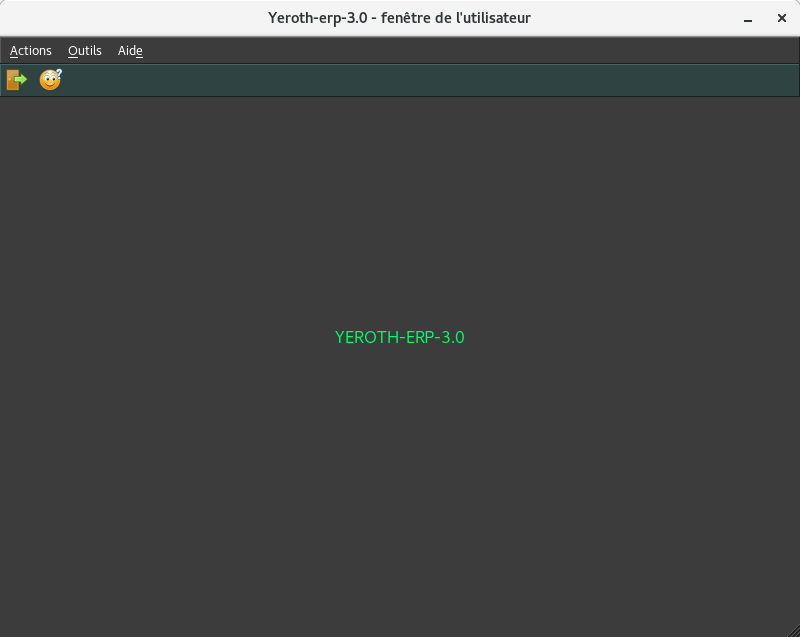
\includegraphics[scale=0.63]{images/yeren-fenetre-principale.png}
\caption{La fen\^etre d'acceuil sans aucun utilisateur enregistr\'e.}
\label{fig:fenetre-principale-utilisateur-non-enregistre}
\end{figure}

\section{Acc\`es au guide de l'utilisateur}

La figure~\ref{fig:fenetre-principale-utilisateur-non-enregistre}
illustre la fen\^etre d'accueil de \yeren sans aucun utilisateur
enregistr\'e.

Il est requis qu'un utilisateur soit enregistr\'e
dans \yeren afin d'avoir acc\`es au manuel de l'utilisateur.

L'utilisateur de \yeren doit accomplir les op\'erations
suivantes afin d'avoir acc\`es au manuel de l'utilisateur:
\begin{enumerate}[1)]
	\item \`a partir de la fen\^etre d'accueil
		(voir figure~\ref{fig:fenetre-principale-utilisateur-non-enregistre}),
		cliquez sur le menu d\'eroulant '\textbf{Aide}'
	\item ensuite cliquez sur le lien '\textbf{Guide de l'utilisateur (PDF)}'.
\end{enumerate}

\section{Structure du guide de l'utilisateur}
Ce manuel de  l'utilisateur de \yeren est structur\'e
comme suit:

\begin{itemize}[\mycheckmark{purplish}]
	\item le chapitre~\ref{chap:utilisateurs} d\'ecrit
	les utilisateurs de \yeren et leurs \roles
	     
	\item le chapitre~\ref{chap:gestion-stocks} explicite
	les fonctionalit\'es de gestion des stocks

	\item le chapitre~\ref{chap:gestion-des-achats} parle
	de la gestion des achats
	
	\item le chapitre~\ref{chap:systeme-dalertes}
	pr\'esente le syst\`eme d'alertes sur les stocks
	
	\item le chapitre~\ref{chap:vendre} d\'ecrit comment
	conclure des ventes d'articles
	
	\item le chapitre~\ref{chap:sortir-articles} d\'ecrit
	comment proc\'eder \`a des sorties et transferts de stocks
	
	\item le chapitre~\ref{chap:vente} explicite comment
	rechercher et imprimer les \'etats de ventes d'articles
	
	\item le chapitre~\ref{chap:etats-des-sorties} explicite
	comment rechercher et imprimer les \'etats de sorties ou
	transferts d'articles
	
	\item le chapitre~\ref{chap:tableaux-de-bord} discute
	de la recherche et de la g\'en\'eration des rapports
	commerciaux de l'entreprise
	
	\item le chapitre~\ref{chap:informations-generales}
	explique comment avoir acc\`es aux d\'etails de
	l'utilisateur enregistr\'e, aux informations commerciales
	de l'entreprise, et enfin \`a la version de \yeren que
	l'on utilise
	
	\item le chapitre~\ref{chap:administration-logiciel}
	traite de l'administration du logiciel

	\item le chapitre~\ref{chap:problemes-connues}
	discute des probl\`emes connues de \yeren
	
	\item enfin, le chapitre~\ref{chap:conclusion} conclut
	ce manuel d'utilisation.
\end{itemize}

